\section{Astoria}
\begin{frame}{Measuring AS-level adversaries against Tor}
	\begin{itemize}
		\item Multiple Autonomous Systems (AS) collude with each other
	performing time based attacks and collecting asymmetric data.

		\item Up to 40\% of circuits constructed by the current Tor
	client are vulnerable to AS-level attackers.

		\item Connections  from  China  were  found  to  be  most  vulnerable 
	to AS-level attackers with up to 86\% of
	all  Tor  circuits.
	\end{itemize}
\end{frame}


\begin{frame}{Mitigating AS-level adversaries against Tor}{ASes
correlations}

	Connections between ASes are negotiated as business arrangements.
\begin{figure}
			\centering
			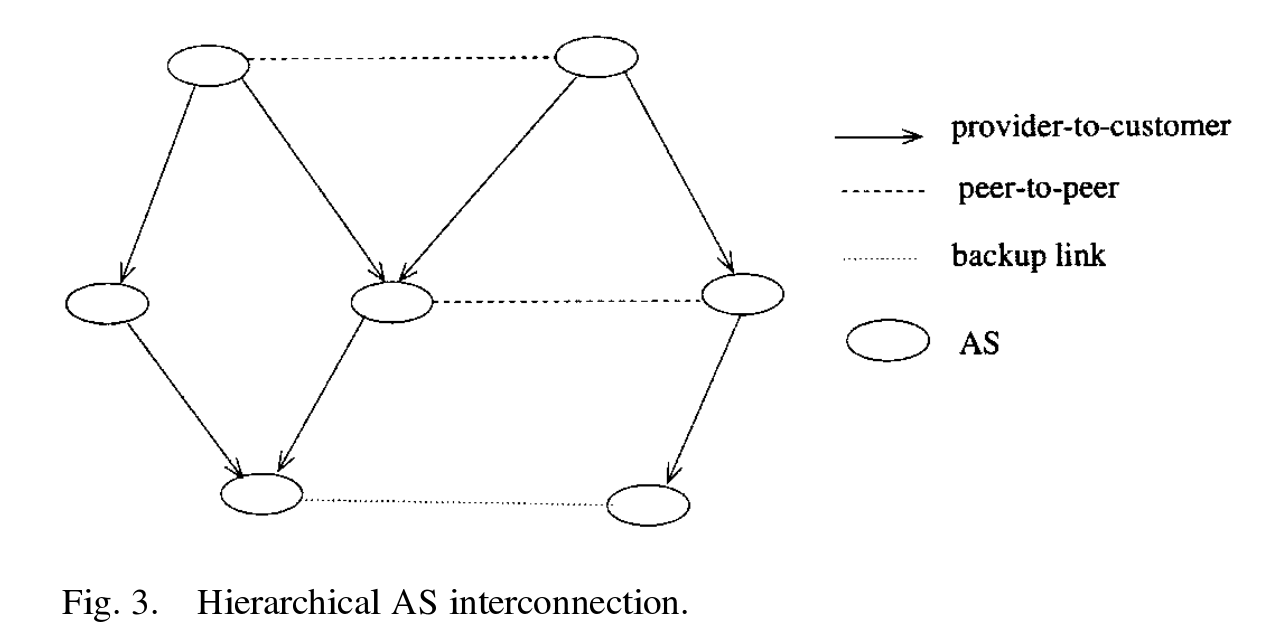
\includegraphics[scale=0.18]{imgs/as_graph.png}
		\end{figure}

	\begin{block}{The idea}
		Building a graph of ASes correlations to identify vulnerable
	paths.
	
	\end{block}
\end{frame}

\begin{frame}{Astoria}

	\begin{itemize}
		\item Use of path prediction to avoid Tor vulnerable paths.\\
	i.e. The entry node and the exit node may be selected together if their ASes 
	are unrelated to each others.
		\item Able to perform  load-balancing at least as well as the vanilla Tor
client.
	\end{itemize}

\end{frame}


%\section{Other ORs and technologies}
%\subsection{HORNET}
	%change OR model
	%faster because does not encrypt the payload for each relay (only
	%the headers)
	%protects also against timing attacks?

\section{Possible Solutions}
\begin{frame}{Possible Solutions}
	User awareness on privacy and anonymity.
	\begin{figure}
		\centering
		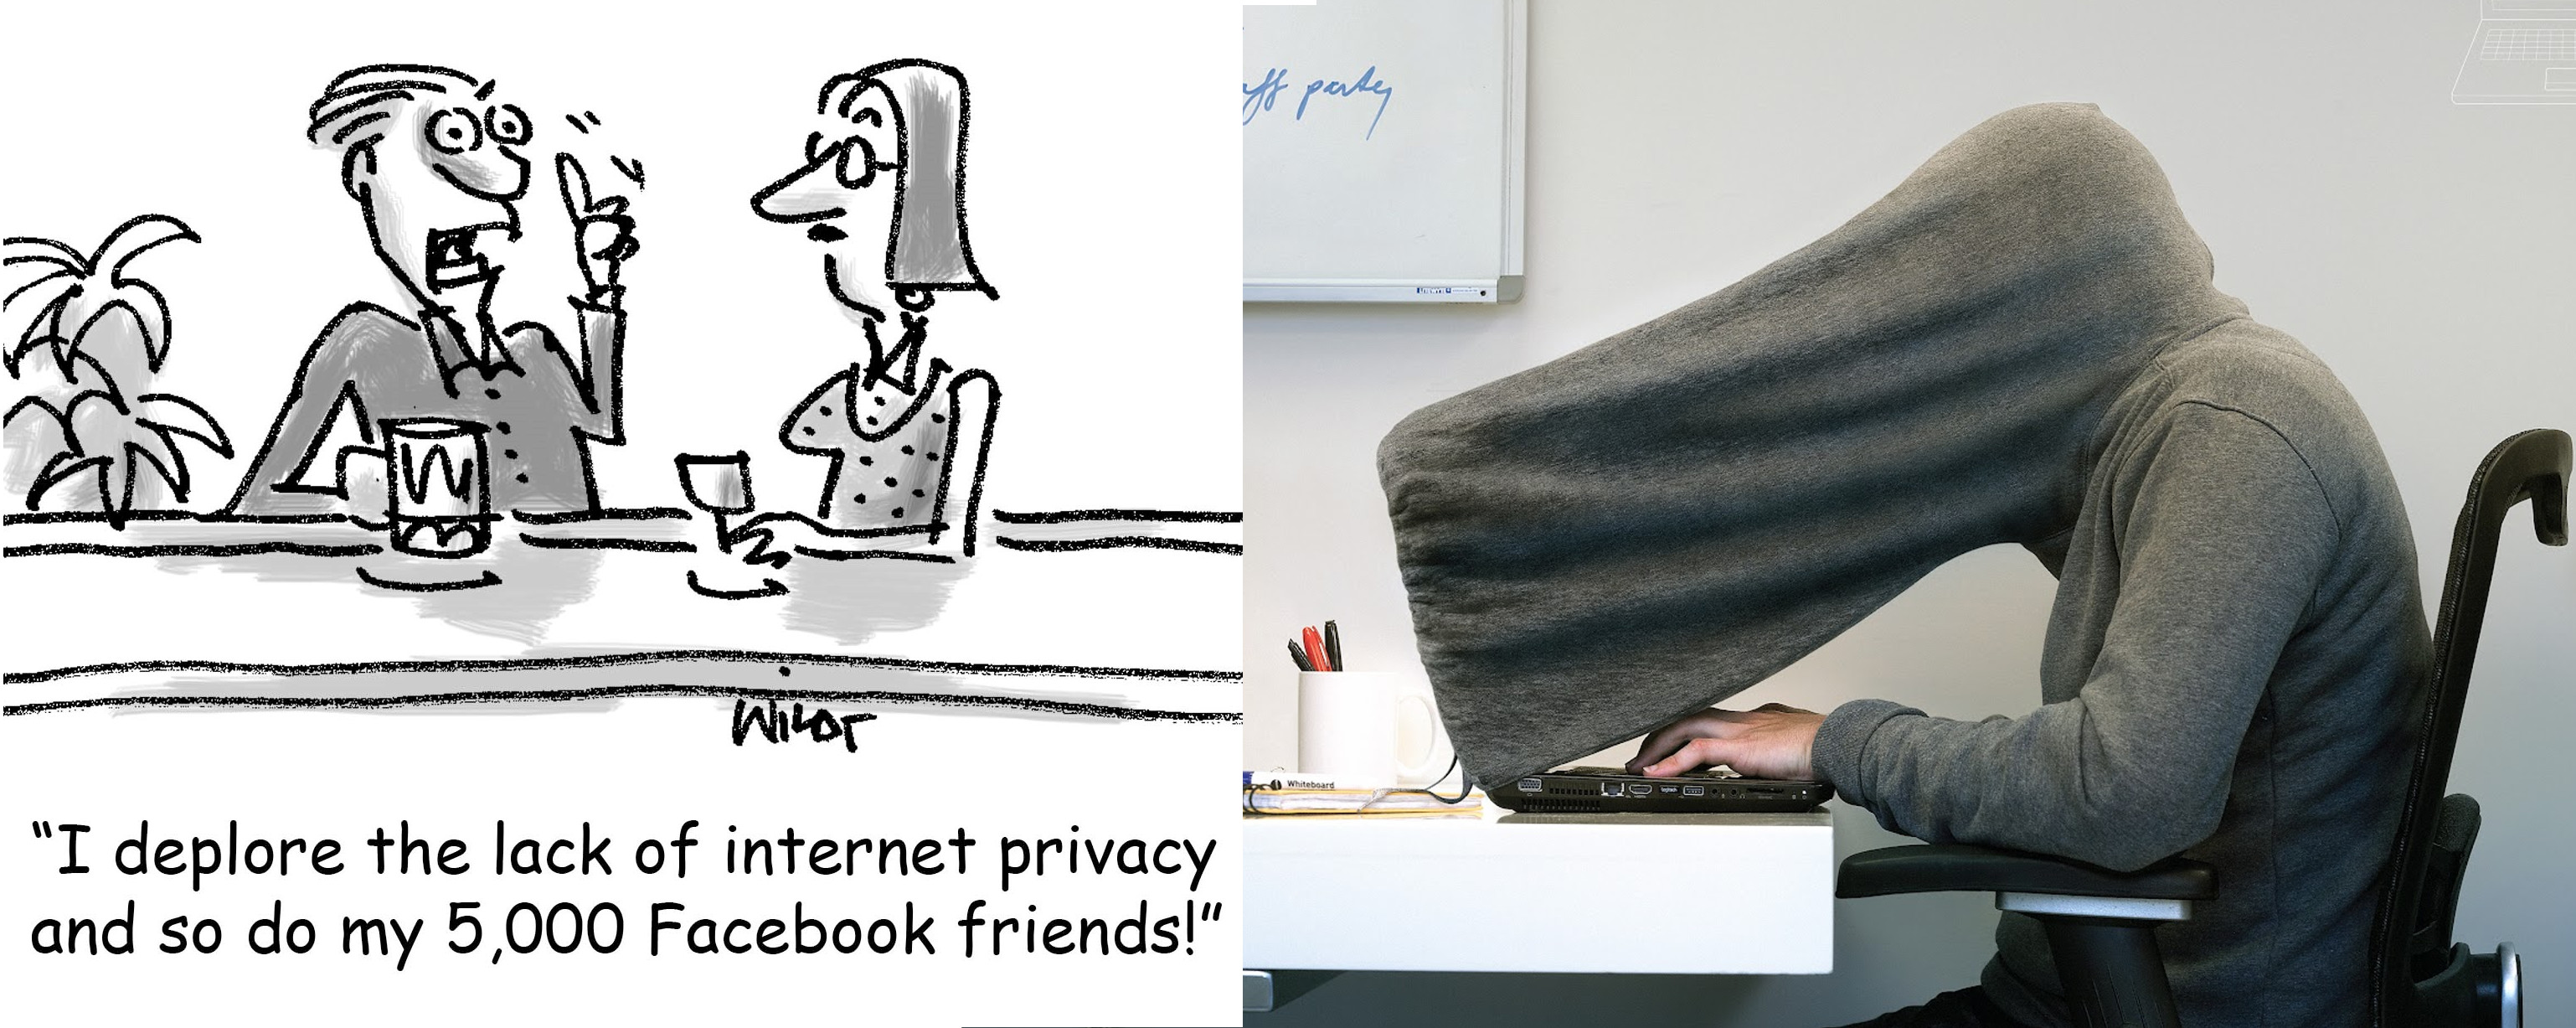
\includegraphics[scale=0.50]{imgs/user_privacy.jpg}
	\end{figure}
\end{frame}

\begin{frame}{Possible Solutions}
	\begin{itemize}
		\item Need of privacy rules reinforcement and more investments on network
security solutions\\
			\small{(i.e. In April 2014, the European Court of Justice declared
invalid the EU Data Retention Directive.)\footnote{According to the directive, 
member states will have to store citizens' telecommunications data for a minimum 
of 6 months and at most 24 months. Under the directive the police and security 
agencies will be able to request access to details such as IP address and time 
of use of every email, phone call and text message sent or received.}}
		\item Academic researches
		\item FOSS
	\end{itemize}	
\end{frame}

